% ============================================================================
%  ICON-MPC -- L4DC 2026 submission
%  Build:  tectonic main.tex     (or: latexmk -pdf main.tex)
%  Use \documentclass[final]{l4dc2026} for the camera-ready version.
% ============================================================================
\documentclass[anon]{l4dc2026}

% amsmath, amssymb, natbib, graphicx, url, algorithm2e are loaded by the class
\usepackage{times}
\usepackage{booktabs}
\usepackage{multirow}
\usepackage{xcolor}
\usepackage{tikz}
\usetikzlibrary{arrows.meta,positioning,fit,calc,shapes.geometric}

% ---------------------------------------------------------------- notation macros
\newcommand{\R}{\mathbb{R}}
\newcommand{\E}{\mathbb{E}}
\newcommand{\1}{\mathbf{1}}
\newcommand{\dhat}{\hat d}
\newcommand{\etil}{\tilde e}
\newcommand{\info}{\mathcal{I}}
\newcommand{\norm}[1]{\left\lVert #1 \right\rVert}
\newcommand{\ours}{ICON-MPC}
\newcommand{\T}{\top}
\DeclareMathOperator*{\argmin}{arg\,min}


\title[ICON-MPC: In-Context Disturbance Estimation for Safe Quadrotor NMPC]{ICON-MPC: In-Context Disturbance Estimation with Gated Delta Networks for Robust, Adaptive and Safe Quadrotor NMPC}

\ifanonsubmission
\author{\Name{Anonymous Authors}}
\else
\author{%
 \Name{Abdelhakim Amer} \Email{hakim.amer@nestai.com}\\
 \addr NestAI
}
\fi

\begin{document}

\maketitle

\begin{abstract}%
Model predictive control (MPC) for quadrotors is only as good as its disturbance estimate, and Kalman-type estimators are optimal only for linear plants, Gaussian noise and known disturbance models. Real flight breaks all three.
We present \ours{}, a nonlinear MPC whose lumped disturbance and filtered state come from an \emph{in-context} Gated Delta Network (GDN) that reads physics residuals and a Kalman-filter bank, behind a learning-free robust front end.
We prove that the gated delta rule is exactly normalised-LMS system identification with forgetting, which diagonal state-space models cannot implement, and that a multi-scale low-pass training loss upper-bounds closed-loop tracking error. Keep-out constraints are tightened by an adaptive conformal margin whose long-run miss rate is bounded for \emph{any} disturbance sequence.
On AdaptiveQuadBench (7 disturbance families $\times$ 8 sensing/fault regimes, 1120 paired trials), \ours{} reduces median tracking error 4--7$\times$ relative to the best of seven stock controllers in every regime except impacts ($p<10^{-6}$), and is significantly better than strengthened KF and multiple-model NMPC baselines under dropout, rotor flicker and combined stress. In obstacle scenarios under combined faults it halves the unsafe-trial rate of constrained baselines (5\% vs.\ 10--16\%), with a realised conformal miss rate of 4.3--5.4\% against a 5\% target.%
\end{abstract}

\begin{keywords}%
  learning-based MPC; in-context estimation; gated delta networks; adaptive conformal prediction; quadrotors; offset-free control
\end{keywords}


\section{Introduction}
\label{sec:intro}

Agile quadrotors operate under disturbances that are hard to model: wind and gusts, payload changes, degraded rotors, unmodelled aerodynamics and contact. Their sensing is also imperfect, with noisy, delayed, dropped or corrupted state estimates.
Two families of controllers dominate. \emph{Adaptive} controllers such as $\mathcal{L}_1$ \citep{hovakimyan2010l1,wu2023l1quad} and INDI \citep{smeur2016adaptive,tal2021accurate} react quickly to a lumped disturbance. However, they act on a single step and ignore constraints. \emph{Model predictive} controllers \citep{sun2022comparative,hanover2022performance,torrente2021data,salzmann2023neuralmpc} plan over a horizon and enforce constraints, but their performance hinges on the disturbance estimate fed to the prediction model. This is the classical offset-free MPC architecture \citep{pannocchia2003disturbance,maeder2009linear}.

\paragraph{When can learning beat a Kalman filter?}
If the plant is linear, the noise Gaussian and the disturbance a known Gauss--Markov process, the Kalman filter (KF) with certainty-equivalent control is optimal (LQG separation). No learned estimator can then do better.
A learned estimator can only win by exploiting violations of these assumptions. Three violations matter here: (i) the operating condition is a \emph{mixture} of regimes with different statistics, so the Bayes estimator is a nonlinear, regime-weighted combination; (ii) the noise is heavy-tailed or contains outliers and dropouts; (iii) the disturbance depends on state and input (e.g., rotor-effectiveness loss scales with thrust), so it is better treated as an unknown \emph{parameter} than as a lumped signal. Here KFs, multiple-model \citep{magill1965optimal,blom1988imm} and outlier-robust KFs \citep{ting2007kalman} must trade one regime against another.

\paragraph{Approach.}
We keep everything that is known exactly and learn only what is not: the NMPC uses the full rigid-body model with rotor drag \citep{faessler2018differential}; a \emph{learning-free} front end handles stale packets, outliers and state jumps; and a sequence model performs \emph{in-context} estimation of the lumped disturbance and the filtered state from physics residuals, as a correction on top of a KF bank.
For the sequence model we use the Gated Delta Network (GDN) \citep{yang2025gated}. We prove that its error-correcting (delta) update is normalised LMS with forgetting, the textbook recursive identification rule, which diagonal state-space models \citep{gu2023mamba} cannot implement; we compare both empirically.
For safety under state constraints, we tighten keep-out constraints by an online \emph{adaptive conformal} margin \citep{gibbs2021adaptive} on the plan-prediction error. The margin carries a distribution-free long-run guarantee.

\paragraph{Contributions.}
\begin{enumerate}
  \item \textbf{Method.} \ours{}: a real-time (${\approx}4$\,ms per step on one CPU thread) offset-free NMPC with an in-context GDN disturbance-and-state estimator, a robust front end and an adaptive conformal safety margin (\S\ref{sec:method}).
  \item \textbf{Guarantees.} (i) the gated delta rule \emph{is} NLMS system identification with forgetting, which diagonal recurrences cannot implement; (ii) a multi-scale low-pass loss upper-bounds closed-loop tracking error; (iii) a distribution-free bound on the long-run frequency of conformal misses and hence of constraint violations (\S\ref{sec:guarantees}).
  \item \textbf{Evidence.} A paired study on AdaptiveQuadBench \citep{zhang2025adaptivequadbench} (1120 trials per controller) against 7 stock and 2 strengthened baselines, plus obstacle scenarios with state constraints and ablations (\S\ref{sec:experiments}). We report where we do \emph{not} win.
\end{enumerate}

\section{Related Work}
\label{sec:related}

\paragraph{Adaptive and robust quadrotor control.}
Geometric control on $SE(3)$ \citep{lee2010geometric} is the standard nominal tracker. $\mathcal{L}_1$ adaptive augmentation \citep{hovakimyan2010l1,wu2023l1quad} and incremental nonlinear dynamic inversion \citep{smeur2016adaptive,tal2021accurate} compensate lumped disturbances at high bandwidth.
Adaptive NMPC \citep{hanover2022performance} and learning-based MPC with GP or neural dynamics \citep{torrente2021data,chee2022knode,saviolo2022pitcn,salzmann2023neuralmpc,bauersfeld2021neurobem,saviolo2024active,scampicchio2025gaussian}, including GPs with dynamic forgetting \citep{amer2025gp} and physics-informed models with control \citep{amer2025pinc}, bring learned compensation into a predictive, constrained framework; NMPC also underpins aerial inspection \citep{amer2023visual} and dynamics emulation on multicopters \citep{amer2026dynamic}. Rotor drag is known to matter at speed \citep{faessler2018differential,sun2022comparative}.
AdaptiveQuadBench \citep{zhang2025adaptivequadbench}, built on RotorPy \citep{folk2023rotorpy}, compares these controllers; we use it unmodified and add sensing/fault regimes and obstacles.

\paragraph{Learning for disturbance adaptation.}
Neural Lander \citep{shi2019neural} and Neural-Fly \citep{oconnell2022neuralfly} learn aerodynamic residuals and adapt a linear head online. RMA \citep{kumar2021rma} and XAdap \citep{zhang2024xadap} learn an adaptation module that infers a latent from history, and XAdap is one of our baselines.
Universal dynamics models \citep{xiao2025anycar} and online continual learning \citep{sarabakha2023online} adapt across platforms and tasks. Learned filters such as KalmanNet \citep{revach2022kalmannet} and Backprop-KF \citep{haarnoja2016backprop} replace or augment the KF gain. \citet{forgione2023incontext} frame system identification as in-context learning across a class of systems.
We take the in-context view inside an offset-free MPC, with a recurrence that is provably a system-identification update and a loss tied to closed-loop error.

\paragraph{Sequence models.}
Selective state-space models (Mamba, \citealp{gu2023mamba}) use input-dependent \emph{diagonal} recurrences. Linear transformers are fast-weight programmers \citep{schlag2021linear}, and the delta rule \citep{widrow1960adaptive} replaces their additive update with an error-correcting one. It can be trained in parallel over the sequence \citep{yang2024parallelizing} and, with gating, gives the Gated Delta Network \citep{yang2025gated}.

\paragraph{Safe learning-based MPC and conformal prediction.}
Learning-based MPC with safety guarantees typically relies on tube constructions \citep{mayne2005robust}, probabilistic constraint tightening \citep{hewing2020cautious,hewing2020learning} or control barrier functions \citep{ames2019cbf}. These require a bound or a distribution on the model error.
Conformal prediction gives distribution-free uncertainty sets. Its adaptive variant (ACI, \citealp{gibbs2021adaptive}; \citealp{angelopoulos2023conformal}) retains long-run coverage under arbitrary distribution shift. It has been used to plan around uncertain \emph{other} agents \citep{lindemann2023safe,dixit2023adaptive}. We instead calibrate the controller's \emph{own} plan-tracking error and use it to tighten soft state constraints \citep{kerrigan2000soft} online.

\section{Problem Setup}
\label{sec:setup}

\paragraph{Dynamics.}
The state is $x=(p,v,q,\omega)\in\R^{13}$: position, velocity, unit quaternion and body rate. The input $u\in[0,f_{\max}]^4$ is the vector of rotor thrusts.
We discretise with step $h=10$\,ms and write the plant as
\begin{equation}
  x_{t+1} = f_\theta(x_t,u_t) + G\, d_t, \qquad d_t = \big(F_t/m,\; J^{-1}\tau_t\big)\in\R^6.
  \label{eq:plant}
\end{equation}
Here $f_\theta$ is the rigid-body model with rotor drag \citep{faessler2018differential,folk2023rotorpy} at nominal parameters $\theta$; the lumped disturbance $d_t$, injected by $G$ into the velocity and body-rate equations, collects \emph{everything else} (wind, external wrench, payload, rotor loss, parameter error).
The controller observes $y_t = \mathcal{S}_t(x_t)$, where the sensing channel $\mathcal{S}_t$ may add Gaussian or heavy-tailed noise, outliers or impacts, or return stale packets (\S\ref{sec:exp-setup}).
Given $y_{1:t}$ and $u_{1:t-1}$, the one-step physics residual
\begin{equation}
  r_t = G^{\dagger}\big(y_{t+1} - f_\theta(y_t,u_t)\big) = d_t + \nu_t
  \label{eq:residual}
\end{equation}
is observable. Here $G^\dagger$ is the left inverse of $G$ and $\nu_t$ collects measurement-noise terms; it is zero-mean under unbiased sensing.

\paragraph{Objective.}
Track a reference $x^{\mathrm{ref}}_t$ with minimal position error $\varepsilon_t = p_t - p^{\mathrm{ref}}_t$. In obstacle scenarios, the controller must also keep the vehicle outside vertical cylinders $\mathcal{O}_j=\{p:\norm{p_{xy}-c_j}\le r_j\}$, where $r_j$ already includes the body radius. Keep-out holds when the clearance satisfies $\min_j(\norm{p_{xy,t}-c_j}-r_j)\ge 0$ for all $t$.
We call a trial \emph{unsafe} if it collides or fails to track (RMSE above 1\,m or divergence).

\section{Method: \ours{}}
\label{sec:method}

\begin{figure}[t]
  \centering
  \resizebox{0.98\linewidth}{!}{% Architecture diagram of ICON-MPC (TikZ, included from sections/04_method.tex)
\begin{tikzpicture}[
  font=\scriptsize, >={Stealth[length=1.6mm]},
  blk/.style={draw, rounded corners=2pt, align=center, minimum height=7mm, inner sep=2pt, fill=#1},
  blk/.default=white, lab/.style={font=\tiny, align=center}]
  \node[blk=gray!12, minimum width=15mm] (plant) {Quadrotor\\(RotorPy)};
  \node[blk=red!8, right=6mm of plant, minimum width=17mm] (fe) {Robust front end\\stale / outlier / jump};
  \node[blk=orange!12, right=6mm of fe, minimum width=16mm] (feat) {Physics features\\residual + KF bank};
  \node[blk=green!15, right=6mm of feat, minimum width=19mm] (gdn) {Gated DeltaNet\\$S_t{=}\alpha_t S_{t-1}(I{-}\beta_t k_tk_t^{\T}){+}\beta_t v_tk_t^{\T}$};
  \node[blk=blue!10, below=7mm of gdn, minimum width=19mm] (mpc) {Offset-free NMPC\\(acados, SQP-RTI)};
  \node[blk=purple!10, left=6mm of mpc, minimum width=16mm] (aci) {Adaptive conformal\\margin $\mu_t$};
  \node[blk=yellow!15, left=6mm of aci, minimum width=17mm] (obs) {Keep-out constraints\\$h_j(p)\ge(r_j{+}\mu_t)^2$};
  \draw[->] (plant) -- node[above, lab]{$y_t$} (fe);
  \draw[->] (fe) -- node[above, lab]{$\bar y_t$} (feat);
  \draw[->] (feat) -- node[above, lab]{$\phi_t$} (gdn);
  \draw[->] (gdn) -- node[right, lab]{$\dhat_t,\ \hat x_t$} (mpc);
  \draw[->] (mpc.south) -- ++(0,-3.5mm) -| node[pos=0.25, below, lab]{rotor thrusts $u_t$} (plant.south);
  \draw[->] (mpc) -- node[above, lab]{plan $\hat X$} (aci);
  \draw[->] (aci) -- (obs);
  \draw[->] (obs.north) -- ++(0,2.5mm) -| ([xshift=-3mm]mpc.north);
  \draw[->, dashed] (fe.south) -- ++(0,-2mm) -| node[pos=0.2, below, lab]{realised $p_t$} (aci.north);
\end{tikzpicture}
}
  \caption{\ours{} architecture. A learning-free front end cleans the telemetry. A Gated DeltaNet reads physics features (one-step residuals and the outputs of a KF bank) and returns the lumped disturbance $\dhat_t$ and a filtered state $\hat x_t$ to an offset-free NMPC. An adaptive conformal margin $\mu_t$, calibrated online on the realised-vs-planned position error, tightens the keep-out constraints.}
  \label{fig:architecture}
\end{figure}

\ours{} (Fig.~\ref{fig:architecture}) has four layers. Each addresses one failure mode and each can be ablated (\S\ref{sec:ablation}).

\subsection{Offset-free nonlinear MPC}
\label{sec:nmpc}
At each tick the controller solves
\begin{equation}
\begin{aligned}
  \min_{x_{0:N},u_{0:N-1},s}\ & \textstyle\sum_{k=0}^{N-1}\big(\norm{x_k-x^{\mathrm{ref}}_k}_Q^2+\norm{u_k-u^{\mathrm{ref}}_k}_R^2\big)+\norm{x_N-x^{\mathrm{ref}}_N}_Q^2+\sum_{k,j}\big(z\,s_{kj}+Z\,s_{kj}^2\big)\\
  \text{s.t.}\ & x_0=\hat x_t,\quad x_{k+1}=F_{\theta}(x_k,u_k;\dhat_t),\quad 0\le u_k\le f_{\max},\\
  & \norm{p_{xy,k}-c_j}^2 \ge (r_j+\mu_t)^2 - s_{kj},\quad s_{kj}\ge 0,\qquad k=1,\dots,N,
\end{aligned}
\label{eq:ocp}
\end{equation}
Here $F_\theta$ integrates \eqref{eq:plant} over one shooting interval with the estimated disturbance $\dhat_t$ held constant over the horizon.
We use a $0.5$\,s horizon with $N=10$ nodes. The solver is acados \citep{verschueren2022acados} with Gauss--Newton SQP-RTI \citep{diehl2005rti}, HPIPM \citep{frison2020hpipm} and explicit Runge--Kutta integration.
The keep-out constraints are soft with an exact $\ell_1$ penalty \citep{kerrigan2000soft} ($z{=}10^3$, $Z{=}10^4$), so the problem is always feasible. Whenever a feasible plan exists, the slack is zero.
The input reference $u^{\mathrm{ref}}_k$ is the static rotor allocation of the flatness-based reference wrench minus the estimated disturbance wrench. This is an offset-free input target \citep{pannocchia2003disturbance,maeder2009linear}: under a constant disturbance and a convergent estimator, the steady-state input matches the disturbance and the tracking offset vanishes.

\subsection{Learning-free robust front end}
Sensor faults are handled \emph{before} any learning, with three rules. \emph{Stale packets} (bit-identical) are flagged, the NMPC dead-reckons $\hat x_t$ with its own model, and estimator kinematics are re-initialised on resume. \emph{Outliers} are rejected when the innovation against the model prediction exceeds $6\times$ a running robust scale plus a floor. \emph{Genuine jumps} (e.g., impacts) are accepted once two consecutive packets agree, followed by a 10-step estimator grace window.

\subsection{In-context disturbance and state estimation with Gated DeltaNet}
\label{sec:gdn}
\paragraph{Features and outputs.}
At each step the network receives a 59-dimensional feature vector $\phi_t$: attitude ($R_t$, 9), velocity (3), body rate (3), rotor speeds (4), the previous normalised input (4), the physics residual $r_t$ of \eqref{eq:residual} (6), kinematic-consistency increments (6), and the outputs of a bank of four lumped KFs (24) tuned for different noise/agility trade-offs.
It outputs a correction to one member of the bank, $\dhat_t = \dhat^{\mathrm{KF}}_t + \sigma_d\odot c_\vartheta(\phi_{1:t})$, together with a filtered state $\hat x_t$ (position, velocity, body rate and an attitude correction) and per-output log-variances.
This \emph{residual parametrisation} contains $c_\vartheta\equiv 0$, so in distribution the population-risk minimiser is never worse than the KF it corrects (App.~\ref{app:proofs}).

\paragraph{Gated delta recurrence.}
Each GDN layer \citep{yang2025gated} maps $\phi_t$ to a key $k_t$ (unit norm), value $v_t$, query $q_t$, decay $\alpha_t\in(0,1)$ and step size $\beta_t\in(0,1)$. It updates a matrix-valued state per head:
\begin{equation}
  S_t = \alpha_t\, S_{t-1}\big(I-\beta_t k_t k_t^{\T}\big)+\beta_t v_t k_t^{\T},\qquad o_t = S_t q_t .
  \label{eq:gdn}
\end{equation}
We use two layers, $d_{\mathrm{model}}=64$ and four heads of dimension 16, for 51k parameters in total.
By Proposition~\ref{prop:nlms}, \eqref{eq:gdn} is normalised LMS with forgetting on $v_t\approx Sk_t$, i.e.\ in-context system identification when keys carry disturbance regressors.
For training we use the exact chunk-parallel form of \eqref{eq:gdn} \citep{yang2024parallelizing} with chunk length 64, which is $14\times$ faster than the sequential scan. At deployment the network runs recurrently, one step per tick, on one CPU thread.

\paragraph{Control-aware training objective.}
Labels are privileged simulator quantities: the mean of the next five noise-free one-step residuals for $d$, and the true state for $\hat x$.
We minimise a heteroscedastic Gaussian negative log-likelihood \citep{kendall2017uncertainties} plus a \emph{multi-scale low-pass} penalty on the error $e_t$:
\begin{equation}
  \mathcal{L} = \textstyle\sum_t \tfrac12\big(e_t^{\T}\Sigma_t^{-1}e_t+\log\det\Sigma_t\big)
  + \lambda \textstyle\sum_{w\in\{10,25,50\}}\sqrt{w}\,\sum_t\norm{\mathrm{MA}_w(e)_t}^2,
  \label{eq:loss}
\end{equation}
where $\mathrm{MA}_w$ is the causal moving average over $w$ steps.
By Theorem~\ref{thm:ms}, such terms upper-bound closed-loop tracking error, whereas per-step MSE does not.
The training data are about $10^4$ five-second rollouts of KF-NMPC behaviour policies over a randomised mixture of regimes, plus one round of DAgger \citep{ross2011dagger} with the learned controller in the loop. The seeds and trial indices are disjoint from the evaluation set.
We train with AdamW \citep{loshchilov2019adamw} and a one-cycle schedule for 40 epochs, three training seeds each. A Mamba \citep{gu2023mamba} and a GRU \citep{cho2014gru} estimator with identical features, outputs and loss serve as architecture controls.

\subsection{Adaptive conformal safety margin}
\label{sec:aci}
The NMPC predicts where the vehicle will be, but noise, faults and estimator error make the realised position deviate from the plan.
Let $\hat p^{(t-\ell)}_{t}$ denote the horizontal position that the plan computed $\ell$ steps earlier predicted for time $t$ (interpolated between nodes; $\ell=10$, two node intervals). The nonconformity score is
\begin{equation}
  e_t = \norm{p_{xy,t}-\hat p^{(t-\ell)}_{t}},
  \qquad
  q_{t+1} = \max\!\big(0,\; q_t+\gamma\,(\1[e_t>q_t]-\alpha)\big),
  \qquad
  \mu_t = \mu_0 + q_t .
  \label{eq:aci}
\end{equation}
This is the quantile-tracking form of adaptive conformal inference \citep{gibbs2021adaptive,angelopoulos2023conformal} with target miss rate $\alpha=0.05$, step size $\gamma=5$\,mm and a floor $\mu_0=1$\,cm.
The margin $\mu_t$ inflates every obstacle in \eqref{eq:ocp}; it grows when sensing degrades (Fig.~\ref{fig:aci}) and shrinks when tracking is accurate. Theorem~\ref{thm:aci} and Corollary~\ref{cor:safety} bound the long-run miss and violation frequencies for \emph{any} disturbance sequence.

\section{Guarantees}
\label{sec:guarantees}

We give three results: one on the estimator class, one on the training objective and one on safety. Proofs are in App.~\ref{app:proofs}. Throughout, $\norm{k_t}=1$.

\subsection{The gated delta rule is in-context system identification}

\begin{proposition}[GDN $=$ NLMS with forgetting]
\label{prop:nlms}
Consider the online least-squares problem of predicting $v_t$ from the regressor $k_t$ with a linear map $S$, with instantaneous loss $\ell_t(S)=\tfrac12\norm{v_t-Sk_t}^2$.
\begin{enumerate}
  \item[(a)] The gated delta update \eqref{eq:gdn} is exactly one normalised-LMS (Kaczmarz) step with step size $\beta_t$ on $\ell_t$, applied to the forgotten estimate $\alpha_t S_{t-1}$:
  \[
    S_t=\alpha_t S_{t-1}-\beta_t\nabla\ell_t(\alpha_t S_{t-1}) = \alpha_t S_{t-1}+\beta_t\big(v_t-\alpha_t S_{t-1}k_t\big)k_t^{\T}.
  \]
  In particular, for a linear-in-parameter disturbance channel $d_t=\varphi_t^{\T}\vartheta_t$ observed through the residual $r_t$, choosing $k_t=\varphi_t/\norm{\varphi_t}$ and $v_t=r_t/\norm{\varphi_t}$ makes the row vector $S_t$ the normalised-LMS estimate of $\vartheta_t^{\T}$ with forgetting factor $\alpha_t$ \citep{widrow1960adaptive}.
  \item[(b)] Let the state of a recurrence be a linear embedding of $S$. If two keys $k,k'$ are neither parallel nor orthogonal and $\beta,\beta'\in(0,1]$, the transitions $A=I-\beta kk^{\T}$ and $A'=I-\beta'k'k'^{\T}$ do not commute. Hence no fixed change of coordinates makes all delta-rule transitions diagonal. Diagonal selective SSMs, whose transitions $\mathrm{diag}(a_t)$ always commute, therefore cannot implement \eqref{eq:gdn} in any linear embedding.
\end{enumerate}
\end{proposition}
Rotor-effectiveness loss, mass/inertia errors and drag make $d_t$ linear in unknown parameters with regressors from rotor speeds and velocity (part of our features). A GDN layer can thus identify them in its state, with input-dependent forgetting $\alpha_t$ (fast re-identification after a fault) and step size $\beta_t$ (slow adaptation under noise): the two knobs a fixed-gain KF lacks.

\subsection{A training loss that upper-bounds closed-loop tracking error}
Let $\etil_t=d_t-\dhat_t$. We assume that, around the reference, the nominal NMPC closed loop is locally exponentially stable (standard with terminal ingredients or a sufficiently long horizon), hence locally input-to-state stable with respect to $\etil$ \citep{sontag2008input}. To first order, the tracking error is the output of a stable, linear time-invariant (LTI), multiple-input multiple-output (MIMO) filter, $\varepsilon=T(z)\,\etil$. Because position is a double integrator of acceleration, $T$ is low-pass. Let $H_w(\omega)=\frac{\sin(w\omega/2)}{w\sin(\omega/2)}$ be the frequency response of $\mathrm{MA}_w$, with $H_1\equiv 1$.

\begin{theorem}[Multi-scale loss bound]
\label{thm:ms}
Let $\etil$ be wide-sense stationary and let $\lambda_1>0$, $\lambda_w\ge 0$. Then
\begin{equation}
  \E\norm{\varepsilon_t}^2 \;\le\; c_\lambda\Big(\lambda_1\,\E\norm{\etil_t}^2+\textstyle\sum_{w>1}\lambda_w\,\E\norm{\mathrm{MA}_w(\etil)_t}^2\Big),
  \qquad
  c_\lambda=\sup_{\omega\in[0,\pi]}\frac{\norm{T(e^{i\omega})}_2^2}{\lambda_1+\sum_{w>1}\lambda_w|H_w(\omega)|^2}.
  \label{eq:msbound}
\end{equation}
For per-step MSE alone ($\lambda_w=0$ for $w>1$), $c_\lambda=\norm{T}_{\mathcal{H}_\infty}^2/\lambda_1$, attained at low frequency. Adding low-pass terms reduces $c_\lambda$ by up to a factor $1+\sum_{w>1}\lambda_w/\lambda_1$ at the frequencies where $\norm{T}$ peaks.
\end{theorem}
This explains why estimators with lower per-step error can track \emph{worse}: slow bias hurts tracking but is barely penalised by per-step MSE. Our loss \eqref{eq:loss} is exactly of the form \eqref{eq:msbound}: the likelihood term plays the role of $\lambda_1$ and $w\in\{10,25,50\}$ cover the closed-loop bandwidth.

\subsection{Distribution-free safety from adaptive conformal margins}

\begin{theorem}[Long-run miss rate]
\label{thm:aci}
Run \eqref{eq:aci} with any $q_1\ge 0$ on any sequence of scores $e_t\in[0,B]$, which may be chosen adversarially and adaptively. Let $m_t=\1[e_t>q_t]$ and $\bar Q=\max\{q_1,\,B+\gamma(1-\alpha)\}$. Then for every horizon $T$,
\begin{equation}
  \frac1T\sum_{t=1}^T m_t \;\le\; \alpha+\frac{\bar Q}{\gamma T}.
\end{equation}
\end{theorem}
\begin{corollary}[Constraint-violation frequency]
\label{cor:safety}
Suppose the plan computed at time $s=t-\ell$ has zero slack and its interpolated prediction $\hat p^{(s)}_t$ satisfies $\norm{\hat p^{(s)}_t-c_j}\ge r_j+\mu_s$ for all $j$. Then $\min_j\big(\norm{p_{xy,t}-c_j}-r_j\big)\ge\mu_s-e_t$.
If in addition $\mu_0\ge\ell\gamma(1-\alpha)$, a collision at time $t$ implies a miss $m_t=1$. Consequently, the long-run fraction of time spent in collision is at most $\alpha+\bar Q/(\gamma T)+\rho_{\mathrm{slack}}$, where $\rho_{\mathrm{slack}}$ is the fraction of plans with nonzero slack.
\end{corollary}
Theorem~\ref{thm:aci} is a long-run frequency statement, not a per-trial bound; we use $\mu_0=1$\,cm $<\ell\gamma(1-\alpha)$ and report empirical frequencies (App.~\ref{app:proofs}).

\section{Experiments}
\label{sec:experiments}

\subsection{Setup}
\label{sec:exp-setup}
\paragraph{Benchmark.}
We use AdaptiveQuadBench \citep{zhang2025adaptivequadbench} with RotorPy \citep{folk2023rotorpy} at 100\,Hz, on 5\,s random trajectories and its seven disturbance families: none, wind, external force, external torque, payload, rotor-effectiveness loss and parameter uncertainty.
For each family we run 20 trials with the benchmark's evaluation seed. Each regime therefore has 140 \emph{paired} trials, in which every controller sees the same vehicle, trajectory, disturbance and noise realisation.
On top of the benchmark we add seven sensing/fault regimes (details in App.~\ref{app:impl}): \emph{noise} (mocap/IMU-level Gaussian noise on all states and rotor speeds); \emph{heavy} (Student-$t$, $\nu{=}2.5$); \emph{outliers} (noise plus 2\%/step 20$\sigma$ glitches); \emph{dropout} (noise plus frozen packets of 50--200\,ms); \emph{impacts} (three kicks of 0.5--1.5\,m/s and 2--5\,rad/s); \emph{rotor flicker} (one rotor toggles between healthy and 30--60\% effectiveness every 0.2--0.8\,s); and \emph{stress} (all of the above with aggressive trajectories).

\paragraph{Baselines.}
\emph{Stock:} the seven controllers shipped with the benchmark, \emph{unmodified}: geometric \citep{lee2010geometric}, geometric-adaptive, $\mathcal{L}_1$-geometric \citep{wu2023l1quad}, adaptive INDI \citep{smeur2016adaptive,tal2021accurate}, MPC, $\mathcal{L}_1$-MPC and the learned XAdap \citep{zhang2024xadap}.
\emph{Strengthened:} because the stock controllers turn out to be far from \ours{}, we also built two strong baselines. They share \emph{everything} with \ours{} (NMPC, rotor-drag model, front end, offset-free input target) except the estimator: a tuned outlier-robust lumped KF \citep{ting2007kalman}, and multiple-model adaptive estimation (MMAE) \citep{magill1965optimal} over the same four-KF bank with forgetting. They isolate the value of the learned estimator.

\paragraph{Metrics and statistics.}
We report median position RMSE, counting a trial with RMSE $>1$\,m or divergence as a failure that is ranked worst. Comparisons use one-sided Wilcoxon signed-rank tests on the paired trials \citep{wilcoxon1945individual} and exact McNemar tests on paired unsafe outcomes \citep{mcnemar1947note}.
Learned estimators are averaged per trial over three training seeds.

\subsection{Tracking under disturbances and sensing faults}
\label{sec:exp-tracking}


\begin{table}[t]
  \centering\small
  \caption{Median position RMSE [cm] per regime (140 paired trials each). Superscripts give the success rate when below 100\%. Bold marks the best NMPC variant. The gain and wins compare \ours{} (GDN, three-seed mean) with the \emph{best} stock controller in that regime, chosen post hoc; all $p<10^{-6}$ (one-sided Wilcoxon).}
  \label{tab:main}
  \resizebox{\linewidth}{!}{\begin{tabular}{l l r r r r r r r}
\toprule
 & \multicolumn{2}{c}{Best stock controller} & NMPC+ & NMPC+ & \multicolumn{2}{c}{\textbf{ICON-MPC (ours)}} & \multicolumn{2}{c}{GDN vs.\ best stock} \\
\cmidrule(lr){2-3}\cmidrule(lr){6-7}\cmidrule(lr){8-9}
Regime & name & RMSE & rob.\ KF & MMAE & Mamba & GDN & gain & wins \\
\midrule
Base & INDI-A & 3.18 & 0.52 & \textbf{0.40} & 0.41 & 0.46 & 7.0$\times$ & 140/140 \\
Gauss.\ noise & L1-MPC & 3.92 & 1.00 & 1.65 & \textbf{0.91} & 0.97 & 4.1$\times$ & 140/140 \\
Heavy-tail & L1-MPC & 4.50 & 0.98 & 1.26 & \textbf{0.84} & 0.91 & 4.9$\times$ & 140/140 \\
Outliers & XAdap & 6.32 & 1.19 & 1.68 & \textbf{1.15} & 1.18 & 5.3$\times$ & 140/140 \\
Dropout & Geo-adaptive & 12.12$^{\,99\%}$ & 2.31 & 3.60 & \textbf{1.77} & 1.83 & 6.6$\times$ & 140/140 \\
Rotor flicker & INDI-A & 3.64 & 1.11 & 1.11 & \textbf{0.63} & 0.74 & 5.0$\times$ & 140/140 \\
Impacts & MPC & 9.95 & \textbf{5.92$^{\,95\%}$} & 6.00 & 6.52 & 7.04 & 1.4$\times$ & 124/140 \\
Stress (all) & XAdap & 59.30$^{\,73\%}$ & 11.06$^{\,92\%}$ & 11.25$^{\,96\%}$ & 10.36 & \textbf{10.00$^{\,99\%}$} & 5.9$\times$ & 138/140 \\
\bottomrule
\end{tabular}
}
\end{table}

\paragraph{Against the benchmark's controllers.}
Table~\ref{tab:main} (and Fig.~\ref{fig:tracking}, App.~\ref{app:results}) shows that \ours{} reduces the median RMSE by $4.1$--$7.0\times$ relative to the best stock controller in every regime except impacts. It wins 138--140 of 140 paired trials ($p<10^{-6}$).
Under combined stress, the best stock controller (XAdap) succeeds in 73\% of trials and \ours{} in 99\%.
Impacts are the exception ($1.4\times$, 124/140 wins). An impact is a state jump rather than a persistent disturbance, so little remains to be estimated, and all NMPC variants are within 20\% of each other.
Outside impacts, even the strengthened KF baseline is $3.3$--$6.1\times$ better than the best stock controller, which motivates the strengthened comparison.


\paragraph{Against strengthened baselines.}
Here only the estimator differs (Table~\ref{tab:main}; per-regime tests in Table~\ref{tab:strong}, App.~\ref{app:results}). The learned estimator is significantly better where the KF assumptions break hardest: packet dropout ($1.26\times$, 117/140 wins), rotor flicker ($1.50\times$; a switching, input-dependent disturbance, the setting of Proposition~\ref{prop:nlms}) and combined stress ($1.11\times$, with success rising from 92.1\% (KF) and 96.4\% (MMAE) to 98.6\%).
The gains are smaller but significant under Gaussian noise, heavy-tailed noise and outliers ($1.01$--$1.07\times$, $p\le 0.013$).
\ours{} does \emph{not} win in two regimes. In the nominal base regime, MMAE is better ($0.87\times$): with clean sensing a bank of well-tuned KFs is near-optimal (Fact~1 in App.~\ref{app:proofs}). Under impacts, the robust KF is better ($0.84\times$) because it reacts to state jumps more conservatively.
Mamba matches or slightly beats GDN in most regimes (per-seed results in App.~\ref{app:results}). We thus do \emph{not} claim GDN is the better drop-in sequence model; its distinguishing feature is the structure of Proposition~\ref{prop:nlms}.

\paragraph{Compute.}
\ours{} takes 3.9\,ms per step on average (6.5\,ms at the 99th percentile) on one CPU thread, within the 10\,ms budget. Stock controllers are $10\times$ cheaper but far less accurate (Table~\ref{tab:compute}, App.~\ref{app:results}).

\subsection{Safety under state constraints: obstacles that intrude into the path}
\label{sec:exp-obstacles}

\paragraph{Scenario.}
We place four vertical cylinders (radius 0.1--0.3\,m plus a 0.1\,m body radius) at least 15\,cm apart, such that the reference \emph{cuts 3--10\,cm into each inflated obstacle}. Tracking the reference blindly therefore guarantees a collision, and the controller must trade tracking for clearance.
We test four regimes: base, noise, rotor flicker and stress (noise, outliers, dropout and flicker together), each with 140 paired trials. The stock controllers have no constraint interface and are shown for reference only.
The constrained baselines use the same soft constraints \eqref{eq:ocp} with either no margin, a fixed 3\,cm margin, or the ACI margin \eqref{eq:aci}.

\begin{figure}[t]
  \centering
  \begin{minipage}[c]{0.66\linewidth}
    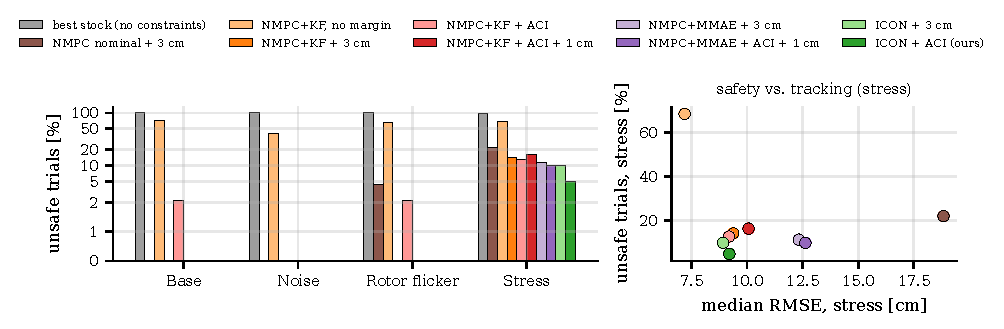
\includegraphics[width=\linewidth]{figures/obstacle_safety.pdf}
  \end{minipage}\hfill
  \begin{minipage}[c]{0.32\linewidth}
    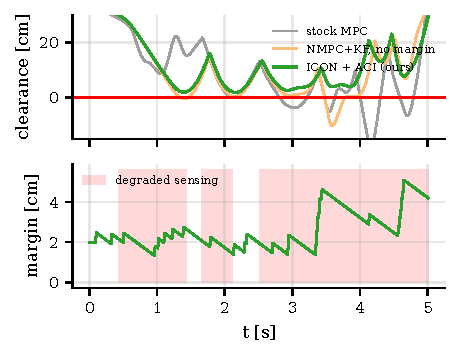
\includegraphics[width=\linewidth]{figures/aci_margin.pdf}
  \end{minipage}
  \caption{\emph{Left:} unsafe-trial rate (collision or failure; symlog scale) and the safety--tracking trade-off under stress. \emph{Right:} one stress trial (wind). Top: clearance to the nearest inflated obstacle; below the red line is a collision. Bottom: the ACI margin $\mu_t$ of \ours{}, which grows during degraded-sensing episodes (shaded) and decays afterwards.}
  \label{fig:obstacles}\label{fig:aci}
\end{figure}


\paragraph{Results.}
\emph{Constraints and margins are necessary:} the stock controllers collide in essentially every trial, and the constrained KF-NMPC without a margin is unsafe in 41--73\% of trials, because noise and estimation error push the realised trajectory over the boundary the plan merely touches.
\emph{Without combined faults, every calibrated margin suffices:} with base, noise or flicker sensing, every margin of 3\,cm or ACI\,+\,1\,cm is safe in all 140 trials, and among these \ours{} tracks best (6.2, 8.0 and 6.3\,cm) because its margin shrinks when tracking is accurate.
\emph{Under combined faults, \ours{} is the safest:} under stress, \ours{} is unsafe in 5.0\% of trials versus 10.0--22.1\% for every other constrained controller (Table~\ref{tab:obstacles}, App.~\ref{app:results}). This is significant against all KF-based and nominal variants, including KF\,+\,ACI with the same floor (16.4\%, $p=2\cdot10^{-4}$), and against MMAE with a 3\,cm margin ($p=0.04$). Against MMAE\,+\,ACI\,+\,1\,cm (10.0\%) the difference is not significant ($p=0.08$), but that baseline tracks 37\% worse (12.6 vs.\ 9.2\,cm). Time in collision falls to 0.07\%, from 0.27\% (MMAE\,+\,ACI) and 0.46\% (KF\,+\,ACI\,+\,1\,cm).
\emph{Calibration matches the theory:} the realised ACI miss frequency is 4.3--5.4\% in every regime and for every estimator, against the target $\alpha=5\%$, as predicted by Theorem~\ref{thm:aci}. The estimator matters because it makes the plan \emph{more predictable}, so the same coverage needs a smaller margin. Figure~\ref{fig:snapshots} (App.~\ref{app:results}) shows a 3D rollout.

\subsection{Ablations}
\label{sec:ablation}
Table~\ref{tab:ablation} (App.~\ref{app:results}) shows that an NMPC \emph{without} disturbance estimation (4--5\,cm, even with rotor drag) is no better than the best stock controller; offset-free estimation with the robust KF alone gives $2.2$--$7.7\times$. Sequence models add on top where KF assumptions fail, and only the selective ones (Mamba, GDN) also help with clean sensing. Removing the front end is catastrophic under dropout (81\% success) and stress (58\%).

\section{Discussion and Limitations}
\label{sec:discussion}
With clean sensing a tuned KF bank is near-optimal (Fact~1, App.~\ref{app:proofs}); the learned estimator pays off (up to $1.5\times$) where KF assumptions fail. All results are in simulation with our own fault models, and the theory is local (Theorem~\ref{thm:ms}). The safety guarantee is a long-run frequency; a hard bound would need a tube \citep{mayne2005robust} with a certified disturbance bound, unavailable for unbounded sensor faults. GDN and Mamba perform similarly; exploiting Proposition~\ref{prop:nlms} more directly is future work.

\section{Conclusion}
\label{sec:conclusion}
\ours{} couples offset-free NMPC, a robust front end, an in-context GDN estimator and an adaptive conformal margin. It tracks $4$--$7\times$ better than the benchmark's controllers, beats strong classical estimators where their assumptions break, and halves unsafe trials under combined faults. Hardware validation is next.


% \acks{Acknowledgements are hidden in the anonymous version.}

\bibliography{references}

\clearpage
\appendix
\section{Proofs and Supporting Facts}
\label{app:proofs}

\paragraph{Fact 1 (no free lunch).}
If the plant is linear, the process and measurement noise are Gaussian with known covariances, and $d_t$ is a Gauss--Markov process matching the KF model, then the KF estimate is the conditional mean $\E[d_t\mid\info_t]$. By the separation principle, certainty-equivalent LQ control with it is optimal for the quadratic cost. Any gain from learning must therefore come from violating one of these assumptions.

\paragraph{Fact 2 (mixtures).}
Let the task distribution be a mixture over regimes $m\in\{1,\dots,M\}$, each linear-Gaussian with Kalman estimate $\dhat^{(m)}_t$. Then
\[
  \E[d_t\mid\info_t]=\sum_m \pi_t(m)\,\dhat^{(m)}_t,\qquad \pi_t(m)=\Pr(m\mid\info_t).
\]
The weights $\pi_t$ are nonlinear functions of the data (likelihood ratios of the innovations). This posterior mean is the unique $L_2$-optimal estimator, so whenever it is not a linear function of the data, every linear time-invariant filter, including any single KF, has strictly larger risk. MMAE implements this posterior under its own (approximate) model. A sequence model trained on samples from the mixture approximates it without requiring the regime models.

\paragraph{Fact 3 (residual parametrisation).}
With $\dhat=\dhat^{\mathrm{KF}}+c_\vartheta$ and a class that contains $c\equiv0$, the population-risk minimiser over the class has risk no larger than the KF. Empirical-risk minimisation adds only the usual generalisation term.

\paragraph{Proof of Proposition~\ref{prop:nlms}.}
(a) With $\ell_t(S)=\frac12\norm{v_t-Sk_t}^2$ we have $\nabla\ell_t(S)=-(v_t-Sk_t)k_t^{\T}$. Hence
\[
\alpha_tS_{t-1}-\beta_t\nabla\ell_t(\alpha_tS_{t-1})=\alpha_tS_{t-1}+\beta_tv_tk_t^{\T}-\alpha_t\beta_tS_{t-1}k_tk_t^{\T}=\alpha_tS_{t-1}(I-\beta_tk_tk_t^{\T})+\beta_tv_tk_t^{\T},
\]
which is \eqref{eq:gdn}. Since $\norm{k_t}=1$, the step is normalised, and $\beta_t=1$ projects onto $\{S:Sk_t=v_t\}$ (Kaczmarz).
For a scalar channel with $r_t=\varphi_t^{\T}\vartheta+\nu_t$, set $k_t=\varphi_t/\norm{\varphi_t}$ and $v_t=r_t/\norm{\varphi_t}$. The update becomes $S_t=\alpha_tS_{t-1}+\beta_t(r_t-\alpha_tS_{t-1}\varphi_t)\varphi_t^{\T}/\norm{\varphi_t}^2$, which is NLMS with leakage (forgetting) $\alpha_t$.

(b) Write $A=I-\beta kk^{\T}$ and $A'=I-\beta'k'k'^{\T}$. Then
\[
AA'=I-\beta kk^{\T}-\beta'k'k'^{\T}+\beta\beta'(k^{\T}k')\,kk'^{\T},\qquad
A'A=I-\beta kk^{\T}-\beta'k'k'^{\T}+\beta\beta'(k^{\T}k')\,k'k^{\T},
\]
so $AA'-A'A=\beta\beta'(k^{\T}k')(kk'^{\T}-k'k^{\T})$. This is nonzero if $k^{\T}k'\neq0$ and $k\not\parallel k'$.
The state transition of \eqref{eq:gdn} acting on $S$ is $S\mapsto\alpha S A$, that is, $\alpha(A^{\T}\otimes I)$ on $\mathrm{vec}(S)$, which inherits the non-commutativity.
Let $M_A=\alpha(A^{\T}\otimes I)$ and suppose an injective linear map $E$ (into a space of any dimension) satisfies $EM_A=D_AE$ and $EM_{A'}=D_{A'}E$ with diagonal $D_A,D_{A'}$. Then $E(M_AM_{A'}-M_{A'}M_A)=(D_AD_{A'}-D_{A'}D_A)E=0$, and injectivity of $E$ gives $M_AM_{A'}=M_{A'}M_A$, contradicting non-commutativity. \hfill$\blacksquare$

\paragraph{Proof of Theorem~\ref{thm:ms}.}
For a stable LTI MIMO system $T$ driven by a wide-sense stationary input with spectral density matrix $S_{\etil}(\omega)\succeq0$, the output covariance satisfies
\[
\E\norm{\varepsilon_t}^2=\frac1{2\pi}\int_{-\pi}^{\pi}\mathrm{tr}\big(T(e^{i\omega})S_{\etil}(\omega)T(e^{i\omega})^*\big)d\omega\le\frac1{2\pi}\int_{-\pi}^{\pi}\norm{T(e^{i\omega})}_2^2\,\mathrm{tr}S_{\etil}(\omega)\,d\omega,
\]
using $\mathrm{tr}(TST^*)\le\norm{T}_2^2\,\mathrm{tr}S$ for $S\succeq0$. Each $\mathrm{MA}_w$ acts componentwise with scalar response $H_w$, so $\E\norm{\mathrm{MA}_w(\etil)_t}^2=\frac1{2\pi}\int|H_w|^2\mathrm{tr}S_{\etil}\,d\omega$.
By the definition of $c_\lambda$, we have $\norm{T}_2^2\le c_\lambda(\lambda_1+\sum_{w>1}\lambda_w|H_w|^2)$ pointwise, and integrating gives \eqref{eq:msbound}. The supremum is finite because $\lambda_1>0$.
Without the $\lambda_1$ term, $c_\lambda$ can be infinite: all $H_w$ with $w\in\{10,25,50\}$ vanish at $\omega=2\pi j/5$, which is why the per-step (likelihood) term is kept. \hfill$\blacksquare$

\paragraph{Proof of Theorem~\ref{thm:aci}.}
Write $q_{t+1}=q_t+\gamma(m_t-\alpha)+c_t$ with $c_t=\max\{0,-(q_t+\gamma(m_t-\alpha))\}\ge0$.
We first show $q_t\le\bar Q$ for all $t$, by induction. If $q_t>B\ge e_t$, then $m_t=0$ and $q_{t+1}\le q_t$. If $q_t\le B$, then $q_{t+1}\le q_t+\gamma(1-\alpha)\le\bar Q$.
Summing the update over $t=1,\dots,T$ gives $\gamma\sum_t(m_t-\alpha)=q_{T+1}-q_1-\sum_tc_t\le\bar Q$. Dividing by $\gamma T$ proves the claim.
Conversely, if the projection is never active ($c_t\equiv0$), then $\frac1T\sum m_t\ge\alpha-q_1/(\gamma T)$, so the miss rate converges to exactly $\alpha$. \hfill$\blacksquare$

\paragraph{Proof of Corollary~\ref{cor:safety}.}
For every $j$, $\norm{p_{xy,t}-c_j}\ge\norm{\hat p^{(s)}_t-c_j}-\norm{p_{xy,t}-\hat p^{(s)}_t}\ge r_j+\mu_s-e_t$.
From \eqref{eq:aci}, $q_{\tau+1}-q_\tau\le\gamma(1-\alpha)$ for every $\tau$, so $q_t\le q_s+\ell\gamma(1-\alpha)$ and $\mu_s=\mu_0+q_s\ge q_t$ whenever $\mu_0\ge\ell\gamma(1-\alpha)$.
A collision ($\min_j(\norm{p_{xy,t}-c_j}-r_j)<0$) then requires $e_t>\mu_s\ge q_t$, that is, $m_t=1$. Collisions at steps whose plan has nonzero slack are counted in $\rho_{\mathrm{slack}}$. \hfill$\blacksquare$

\paragraph{Scope of the safety guarantee.}
Theorem~\ref{thm:aci} holds for \emph{any} disturbance and fault sequence, but it is a long-run frequency statement, not a hard per-trial bound. The lag condition $\mu_0\ge\ell\gamma(1-\alpha)=4.75$\,cm is a worst case (misses on $\ell$ consecutive steps). We use $\mu_0=1$\,cm, which tracks better, and report the empirical miss and collision frequencies instead (\S\ref{sec:exp-obstacles}). Inter-node chord error is a few millimetres and is absorbed by $\mu_0$.

\subsection{Safe online aggregation}
\label{app:aggregation}
Let experts $j=1..K$ (e.g., robust KF, fast KF, GDN) predict $\dhat^{(j)}_t$ before $r_t$ is revealed, with loss $\ell^j_t=\norm{r_t-\dhat^{(j)}_t}^2$.
If $\nu_t$ is conditionally zero-mean and uncorrelated with the expert predictions (exactly so when predictions use information up to $t-1$, approximately otherwise), $\E\ell^j_t=\E\norm{\etil^{(j)}_t}^2+\E\norm{\nu_t}^2$, so the observable loss ranks the experts by their true estimation error. The regret bound below holds without this assumption.
On a domain with $\norm{r},\norm{\dhat}\le B$, the squared loss is $\eta$-exp-concave with $\eta=1/(8B^2)$. Exponentially weighted averaging therefore guarantees, for \emph{any} sequence, $\sum_t\ell^{\mathrm{mix}}_t\le\min_j\sum_t\ell^j_t+8B^2\ln K$ \citep{cesabianchi2006prediction}.
We implemented this aggregation (\texttt{agg}). It matched the GDN alone, for example 9.7 vs 10.0\,cm median RMSE under stress, so we report the GDN in the main text.

\section{Implementation Details}
\label{app:impl}

\paragraph{NMPC.}
State $x=(p,v,q,\omega)$ with $q$ in $wxyz$ order; inputs are the four rotor thrusts with bounds $[0,f_{\max}]$. The model is the RotorPy wrench model with rotor drag (coefficients $k_d,k_z$, rotor-speed floor 50\,rad/s).
Horizon 0.5\,s with $N{=}10$ nodes; weights $Q=\mathrm{diag}(10\cdot\1_3,\,10\cdot\1_3,\,0.1\cdot\1_4,\,0.01\cdot\1_3)$ and $R=0.01\cdot I_4$, plus a yaw-tracking term.
The solver is acados with SQP-RTI, a Gauss--Newton Hessian, FULL\_CONDENSING\_HPIPM and an explicit Runge--Kutta integrator. Per-stage parameters are $(m,J,r_i,\kappa_i,F_{\mathrm{ext}},\tau_{\mathrm{ext}},\text{wind})$.
Obstacle slots that are not in use are placed 10\,m away; very distant dummy slots degraded the QP scaling.

\paragraph{Estimators.}
The KF bank consists of four lumped random-walk KFs on $(F/m,J^{-1}\tau)$ with different measurement and process noise. The robust-KF baseline uses $r_v{=}r_\omega{=}0.15$, $q_F{=}10$, $q_\tau{=}1$. MMAE combines the bank with posterior forgetting 0.95.
The GDN has 2 layers, $d_{\mathrm{model}}{=}64$, 4 heads of size 16, a short depthwise causal convolution on $q,k,v$, SiLU activations, $\ell_2$-normalised queries and keys, and a SiLU output gate (51k parameters). Mamba has 2 layers, $d_{\mathrm{model}}{=}64$ and $d_{\mathrm{state}}{=}16$ (72k parameters). The GRU has 2 layers with hidden size 64 (56k parameters).
The output head has 36 values: 18 means (6 disturbance corrections and 12 state outputs) and 18 log-variances.
Training: AdamW with learning rate $2\cdot10^{-3}$, one-cycle schedule, batch size 32, 40 epochs, gradient clipping at 1, multi-scale weight $\lambda{=}1$ with windows $\{10,25,50\}$; validation is by held-out trial index. On one RTX~5070 GPU, the chunk-parallel form takes 19\,ms per batch, against 275\,ms for the sequential scan.
Data: KF-NMPC behaviour rollouts (one of several KF tunings chosen per trial) on the training regime mixture, plus one DAgger round. In total ${\approx}10^4$ five-second sequences from benchmark seed 7 and trial indices 20--539, disjoint from evaluation (seed 42, trials 0--19).

\paragraph{Sensing and fault regimes.}
Noise standard deviations: position 5\,mm, velocity 0.05\,m/s, attitude 0.01\,rad, body rate 0.05\,rad/s and rotor speed 20\,rad/s. \emph{Heavy}: the same scales with Student-$t$ ($\nu{=}2.5$) draws.
\emph{Outliers}: with probability 2\% per step and per channel group, a 20$\sigma$ glitch.
\emph{Dropout}: after 0.5\,s, with probability 1\% per step, the controller receives the last packet for 5--20 steps.
\emph{Impacts}: three kicks at uniformly random times in $[1,4.5]$\,s.
\emph{Rotor flicker}: after a random onset, one rotor alternates between healthy and 30--60\% effectiveness every 0.2--0.8\,s.
\emph{Stress}: noise, outliers, dropout, impacts, flicker and aggressive trajectories (position range $\pm4$\,m, velocity and acceleration $\pm6$).
All regime randomness uses dedicated per-trial random streams, so every controller sees identical realisations.

\paragraph{Obstacles.}
Four cylinders with radius $\sim U(0.1,0.3)$\,m plus $R_{\mathrm{body}}=0.1$\,m. Each is placed at a random time $t_k\in[0.8,4.7]$\,s, on a random side of the reference, so that the reference penetrates the inflated cylinder by 3--10\,cm. Cylinders are at least 15\,cm apart, the first 0.8\,s of the reference is collision-free, and placement uses up to 3000 rejection-sampling attempts.
ACI: $\alpha{=}0.05$, $\gamma{=}5$\,mm, $q_1{=}2$\,cm, $\ell{=}10$ steps, floor $\mu_0{=}1$\,cm.

\paragraph{Reproducibility.}
All code (controllers, regimes, training, analysis, figure and table generation) will be released. Every figure and table in this paper is produced by a single script from the raw per-trial CSV files.

\section{Additional Results}
\label{app:results}

\begin{table}[h]
  \centering\small
  \caption{\ours{} (GDN) against the best \emph{strengthened} baseline per regime (same NMPC, front end and input target; only the estimator differs). Gain $=$ median RMSE ratio; one-sided Wilcoxon on 140 paired trials.}
  \label{tab:strong}
  \begin{tabular}{l l r r r}
\toprule
Regime & best strong baseline & GDN gain & wins & $p$ (Wilcoxon) \\
\midrule
Base & MMAE & 0.87$\times$ & 7/140 & 1.00 \\
Gauss.\ noise & robust KF & 1.03$\times$ & 78/140 & $4\!\cdot\!10^{-3}$ \\
Heavy-tail & robust KF & 1.07$\times$ & 83/140 & 0.01 \\
Outliers & robust KF & 1.01$\times$ & 93/140 & $5\!\cdot\!10^{-5}$ \\
Dropout & robust KF & 1.26$\times$ & 117/140 & $<\!10^{-6}$ \\
Rotor flicker & MMAE & 1.50$\times$ & 81/140 & $<\!10^{-6}$ \\
Impacts & robust KF & 0.84$\times$ & 33/140 & 1.00 \\
Stress (all) & robust KF & 1.11$\times$ & 78/140 & $3\!\cdot\!10^{-3}$ \\
\bottomrule
\end{tabular}

\end{table}

\begin{figure}[h]
  \centering
  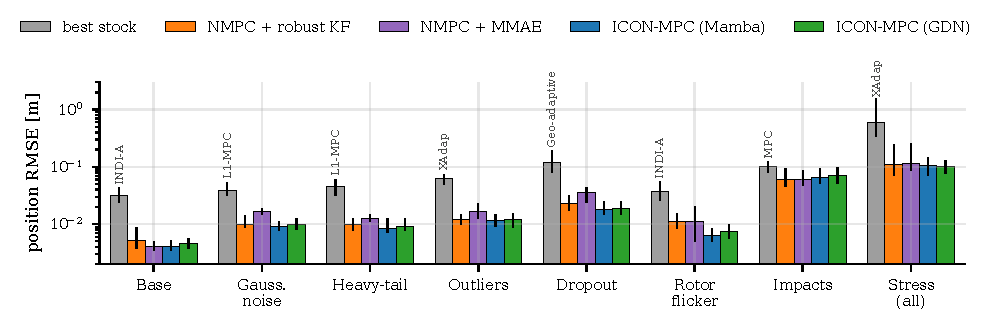
\includegraphics[width=\linewidth]{figures/tracking_results.pdf}
  \vspace{-6mm}
  \caption{Median position RMSE (log scale; whiskers show the inter-quartile range) over 140 paired trials per regime. Grey: best of the seven stock controllers, whose name is shown above the bar. Orange/purple: our strengthened NMPC baselines. Blue/green: \ours{} with Mamba and with GDN estimators.}
  \label{fig:tracking}
\end{figure}

\begin{table}[h]
  \centering\small
  \caption{Obstacle scenarios (140 paired trials each): unsafe-trial rate, median RMSE [cm] and an exact one-sided McNemar test of ``baseline is less safe than \ours{}''.}
  \label{tab:obstacles}
  \begin{tabular}{l rrr rrr}
\toprule
 & \multicolumn{3}{c}{Base (no sensing faults)} & \multicolumn{3}{c}{Stress} \\
\cmidrule(lr){2-4}\cmidrule(lr){5-7}
Controller & unsafe & RMSE & $p$ & unsafe & RMSE & $p$ \\
\midrule
best stock (no constraints) & 100.0\% & 11.8 & $<\!10^{-6}$ & 99.3\% & 17.3 & $<\!10^{-6}$ \\
NMPC nominal + 3 cm & 0.0\% & 10.1 & 1.00 & 22.1\% & 18.8 & $2\!\cdot\!10^{-5}$ \\
NMPC+KF, no margin & 72.9\% & 5.2 & $<\!10^{-6}$ & 68.6\% & 7.2 & $<\!10^{-6}$ \\
NMPC+KF + 3 cm & 0.0\% & 7.6 & 1.00 & 14.3\% & 9.4 & $2\!\cdot\!10^{-3}$ \\
NMPC+KF + ACI & 2.1\% & 5.6 & 0.12 & 12.9\% & 9.2 & $6\!\cdot\!10^{-3}$ \\
NMPC+KF + ACI + 1 cm & 0.0\% & 6.4 & 1.00 & 16.4\% & 10.1 & $2\!\cdot\!10^{-4}$ \\
NMPC+MMAE + 3 cm & 0.0\% & 7.4 & 1.00 & 11.4\% & 12.3 & 0.04 \\
NMPC+MMAE + ACI + 1 cm & 0.0\% & 6.3 & 1.00 & 10.0\% & 12.6 & 0.08 \\
ICON + 3 cm & 0.0\% & 7.5 & 1.00 & 10.0\% & 8.9 & $8\!\cdot\!10^{-3}$ \\
\textbf{ICON + ACI (ours)} & 0.0\% & 6.2 & -- & 5.0\% & 9.2 & -- \\
\bottomrule
\end{tabular}

\end{table}

\paragraph{Ablation and compute.}
Tables~\ref{tab:ablation} and~\ref{tab:compute} support \S\ref{sec:ablation} and the compute paragraph of \S\ref{sec:exp-tracking}.

\begin{table}[h]
  \centering\small
  \caption{Ablation: median RMSE [cm] (140 paired trials per regime; superscript gives the success rate when below 100\%). Upper block: adding components cumulatively. Lower block: removing one component from the full model. All learned rows use training seed 0.}
  \label{tab:ablation}
  \resizebox{\linewidth}{!}{\begin{tabular}{l rrrrrrrr}
\toprule
Variant & Base & Gauss.\ noise & Heavy-tail & Outliers & Dropout & Rotor flicker & Impacts & Stress (all) \\
\midrule
NMPC, nominal model (no drag, no estimator) & 5.08 & 4.89 & 4.98 & 5.08 & 6.08 & 9.45 & 9.52 & 22.72$^{95}$ \\
\quad + rotor-drag model & 4.02 & 4.01 & 3.98 & 4.01 & 5.02 & 8.52 & 8.83 & 20.98$^{94}$ \\
\quad + robust lumped KF & 0.52 & 1.00 & 0.98 & 1.19 & 2.31 & 1.11 & 5.92$^{95}$ & 11.06$^{92}$ \\
\quad + learned estimator: GRU & 0.52 & 1.02 & 1.00 & 1.23 & 1.87 & 0.79 & 6.53 & 9.97$^{98}$ \\
\quad + learned estimator: Mamba & 0.41 & 0.92 & 0.81 & 1.02 & 1.81 & 0.64 & 6.54 & 9.44 \\
\quad + learned estimator: GDN (full) & 0.46 & 0.97 & 0.91 & 1.19 & 1.79 & 0.74 & 7.53 & 9.34$^{98}$ \\
\midrule
full $-$ robust front end & 0.46 & 0.97 & 0.93 & 1.83 & 24.22$^{81}$ & 0.66 & 6.92 & 55.98$^{58}$ \\
full $-$ learned state filter & 0.46 & 0.94 & 0.89 & 1.16 & 1.93 & 0.76 & 7.64 & 9.99$^{99}$ \\
full $-$ offset-free input reference & 0.46 & 0.97 & 0.91 & 1.19 & 1.80 & 0.75 & 7.53 & 9.53$^{99}$ \\
\bottomrule
\end{tabular}
}
\end{table}

\begin{table}[h]
  \centering\small
  \caption{Controller compute per 100\,Hz step (single CPU thread; 30 trials run in parallel) and outcome under stress.}
  \label{tab:compute}
  \begin{tabular}{l r r r r}
\toprule
Controller & mean [ms] & p99 [ms] & stress success & stress RMSE [cm] \\
\midrule
Geometric & 0.42 & 3.3 & 14\% & fail \\
Geo-adaptive & 0.50 & 3.4 & 17\% & fail \\
L1-Geo & 0.63 & 3.7 & 7\% & fail \\
INDI-A & 0.39 & 3.1 & 9\% & fail \\
L1-MPC & 0.54 & 5.5 & 10\% & fail \\
MPC & 0.32 & 3.3 & 59\% & 86.1 \\
XAdap & 0.62 & 5.2 & 73\% & 59.3 \\
\midrule
NMPC + robust KF & 3.59 & 7.4 & 92\% & 11.1 \\
NMPC + MMAE & 4.43 & 9.1 & 96\% & 11.2 \\
\textbf{ICON-MPC (GDN)} & 3.93 & 6.5 & 98\% & 9.3 \\
ICON-MPC (Mamba) & 3.65 & 5.9 & 100\% & 9.4 \\
\bottomrule
\end{tabular}

\end{table}

\paragraph{Training-seed variability.}
Table~\ref{tab:seeds} lists the median RMSE of each training seed. Seed-to-seed variation (up to 15\% under stress) is comparable to the gap between the two selective architectures.

\begin{table}[h]
  \centering\small
  \caption{Median position RMSE [cm] per training seed (140 paired trials per regime).}
  \label{tab:seeds}
  \begin{tabular}{l rrr rrr}
\toprule
 & \multicolumn{3}{c}{GDN seed} & \multicolumn{3}{c}{Mamba seed} \\
\cmidrule(lr){2-4}\cmidrule(lr){5-7}
Regime & 0 & 1 & 2 & 0 & 1 & 2 \\
\midrule
Base & 0.46 & 0.47 & 0.45 & 0.41 & 0.41 & 0.41 \\
Gauss.\ noise & 0.97 & 0.98 & 0.94 & 0.92 & 0.89 & 0.91 \\
Heavy-tail & 0.91 & 0.92 & 0.93 & 0.81 & 0.82 & 0.91 \\
Outliers & 1.19 & 1.18 & 1.14 & 1.02 & 1.13 & 1.13 \\
Dropout & 1.79 & 1.88 & 1.76 & 1.81 & 1.77 & 1.81 \\
Rotor flicker & 0.74 & 0.79 & 0.68 & 0.64 & 0.60 & 0.64 \\
Impacts & 7.53 & 7.07 & 6.65 & 6.54 & 6.53 & 6.48 \\
Stress (all) & 9.34 & 9.76 & 10.30 & 9.44 & 9.37 & 10.77 \\
\bottomrule
\end{tabular}

\end{table}

\paragraph{Qualitative 3D rollouts.}
Figure~\ref{fig:snapshots} shows two stress trials (all faults combined). Animated versions are provided in the supplementary material.

\begin{figure}[h]
  \centering
  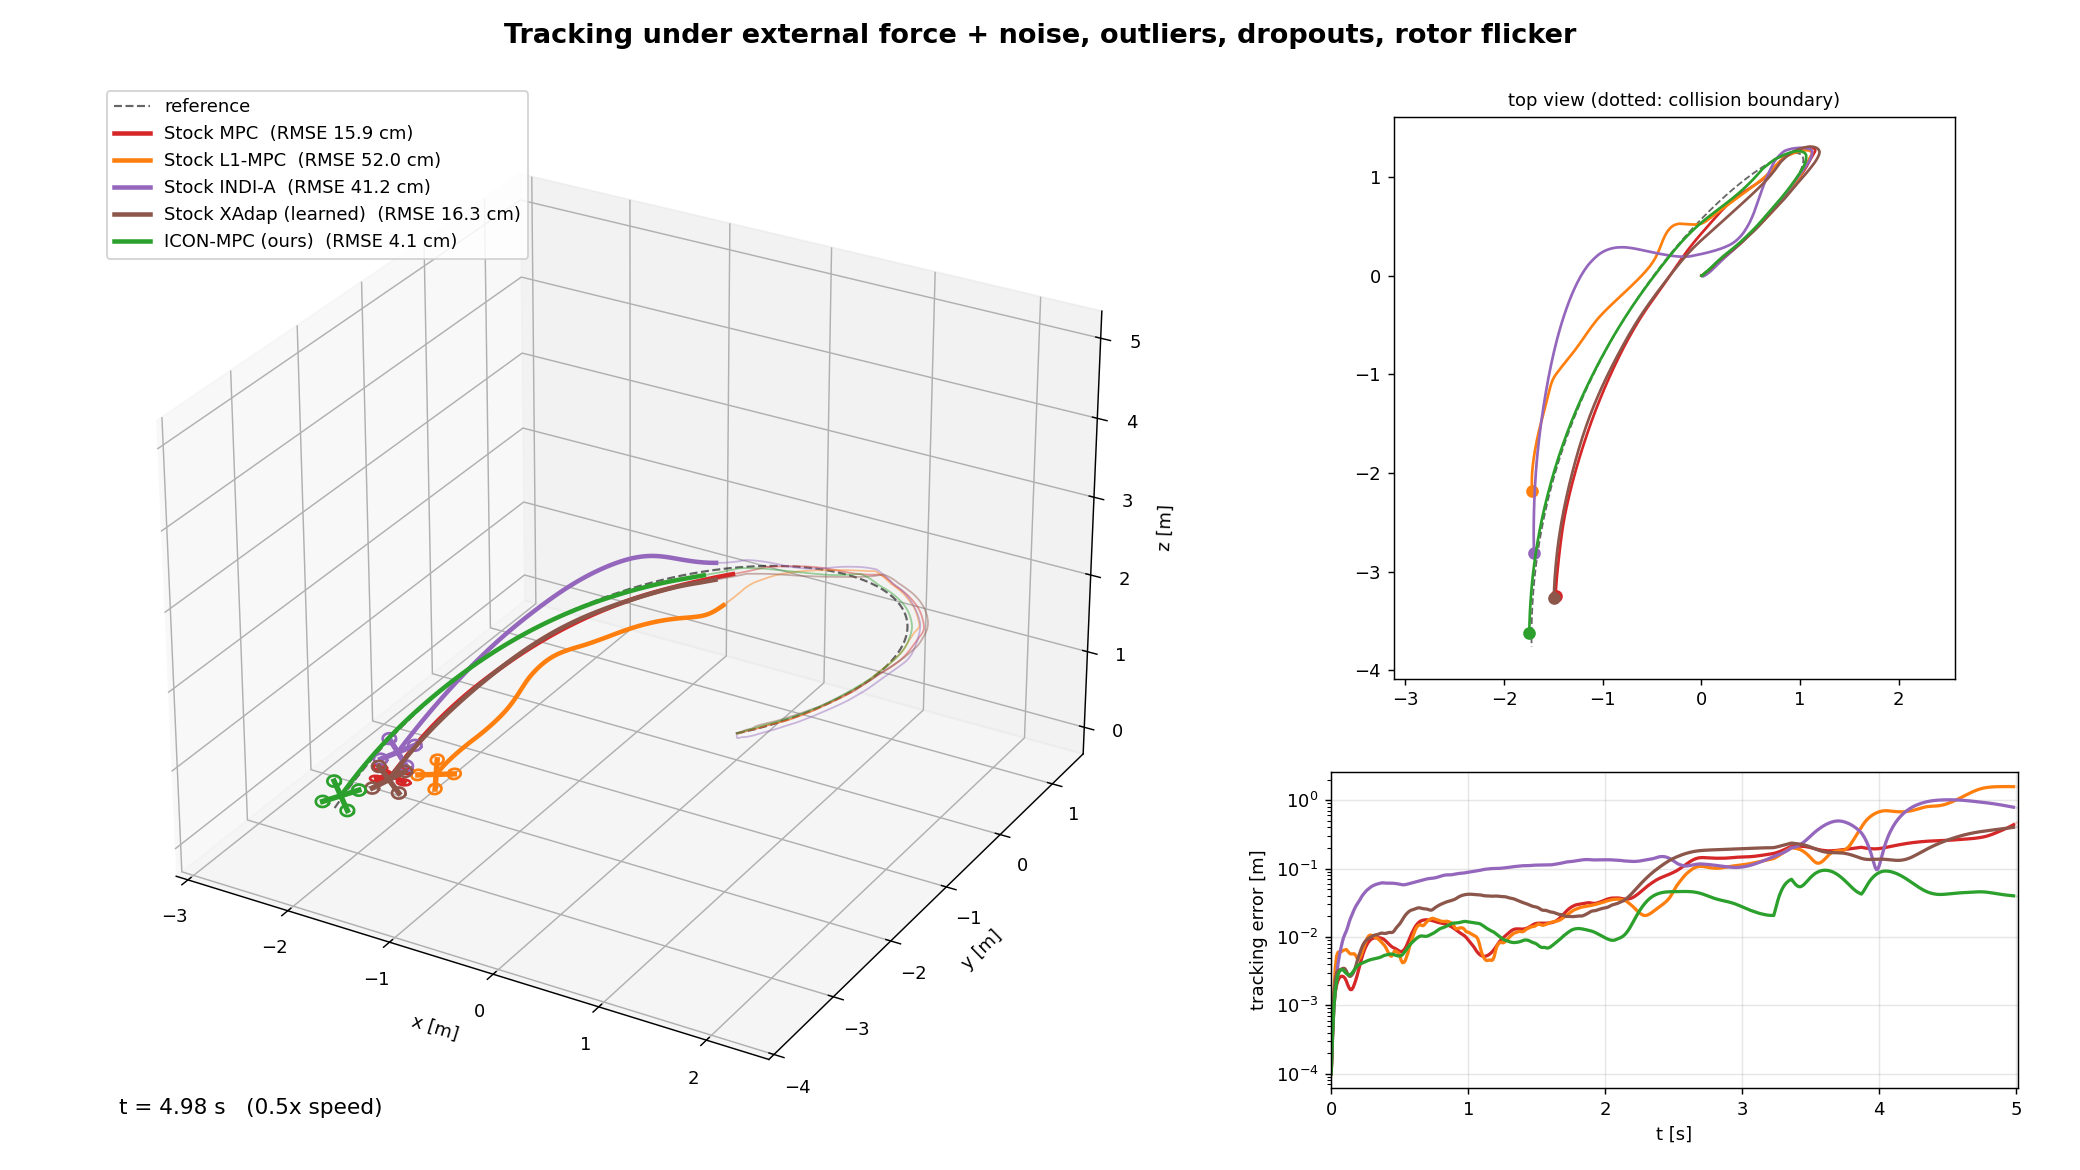
\includegraphics[width=\linewidth]{figures/snapshot_tracking.png}\\[2mm]
  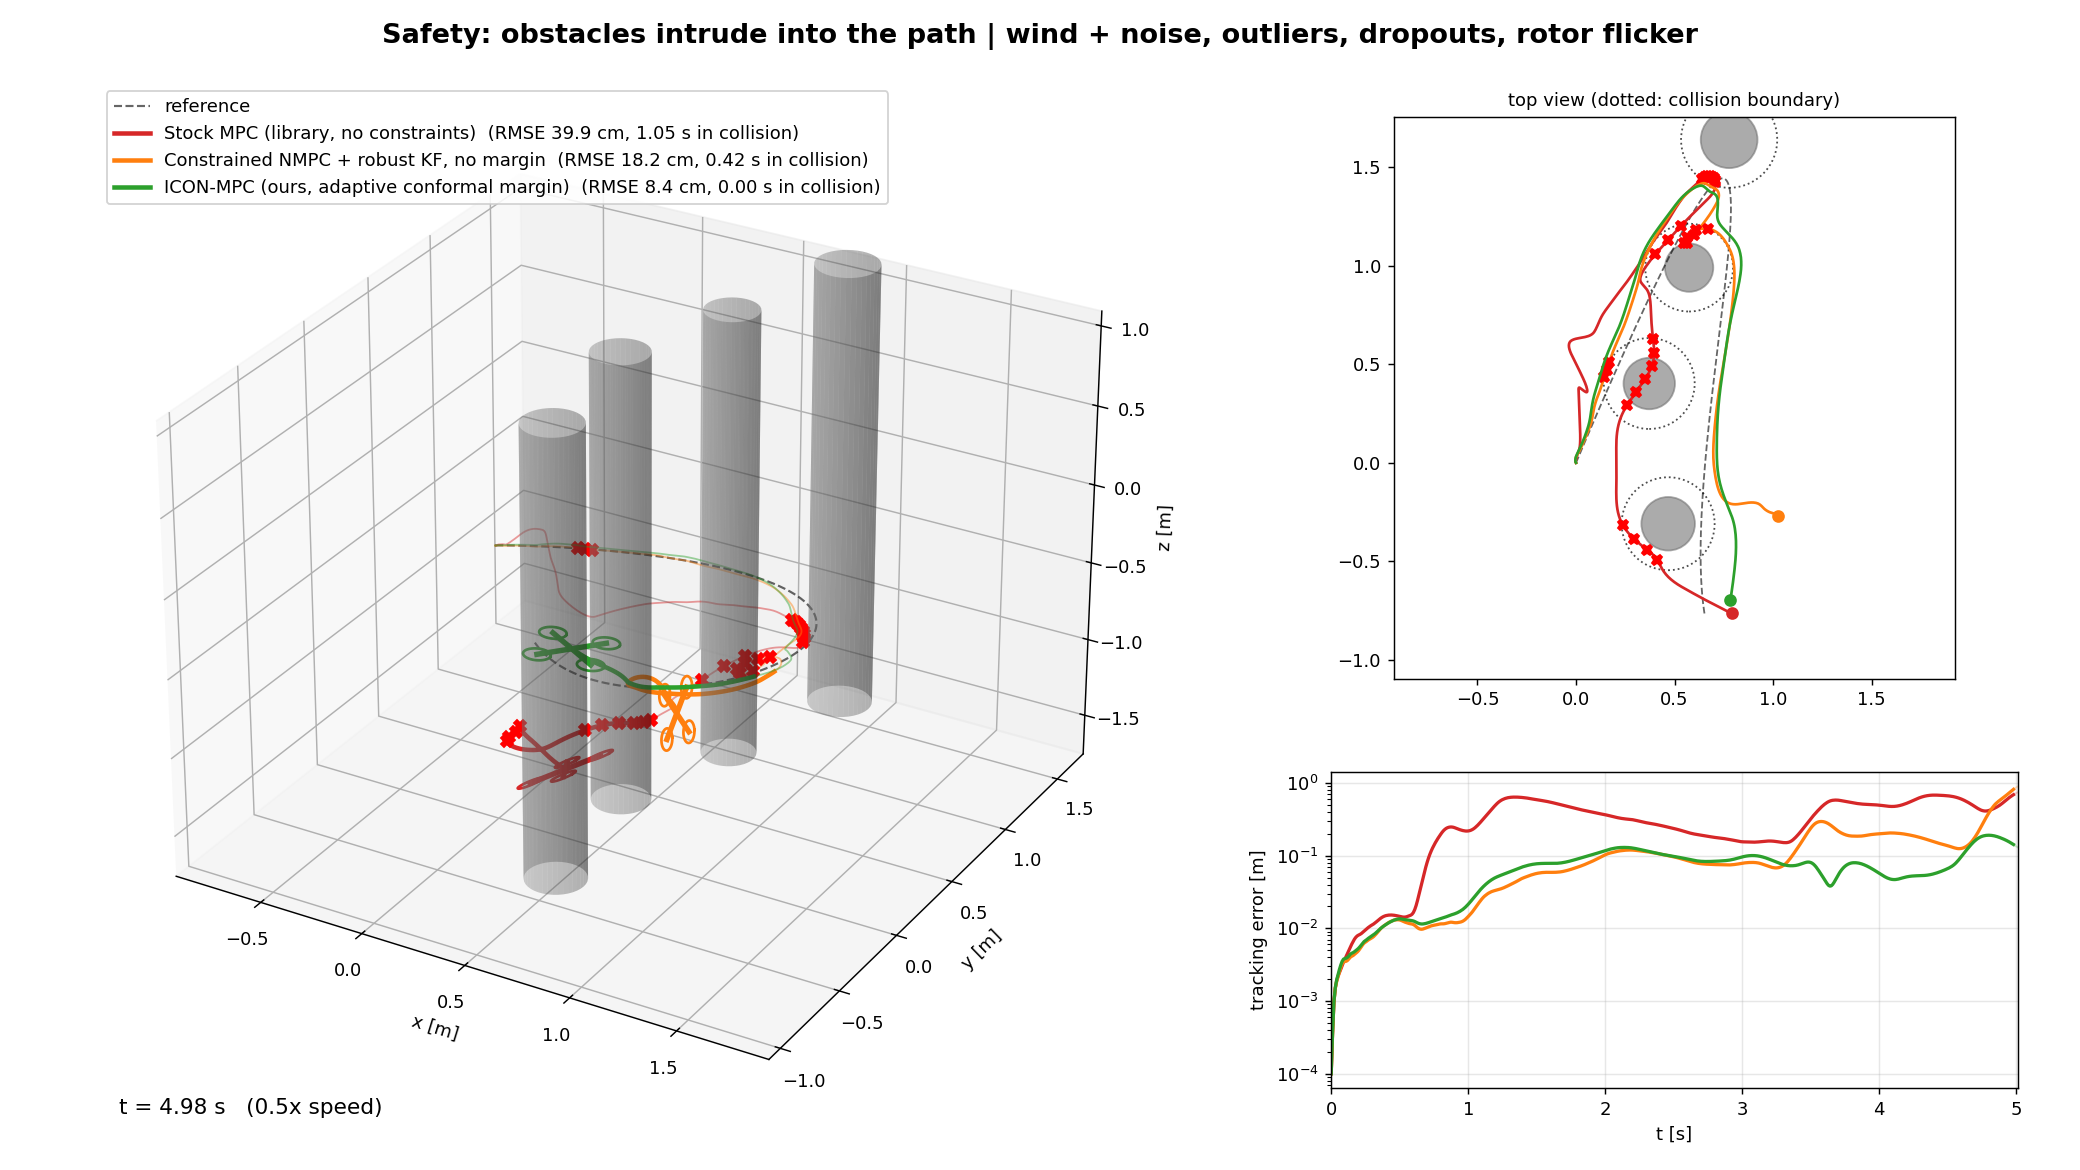
\includegraphics[width=\linewidth]{figures/snapshot_safety.png}
  \caption{\emph{Top:} external force plus stress. \ours{} (green) tracks with 4.1\,cm RMSE, against 15.9--52.0\,cm for the stock MPC, $\mathcal{L}_1$-MPC, INDI-A and XAdap. \emph{Bottom:} wind plus stress, with obstacles intruding into the path (red crosses mark collisions). The stock MPC spends 1.05\,s in collision and the constrained KF-NMPC without a margin 0.42\,s. \ours{} with the conformal margin never collides, with 8.4\,cm RMSE.}
  \label{fig:snapshots}
\end{figure}


\end{document}
